 %
In the three previous sections, we have derived the relationships between liquidity constraints, consumption concavity, and prudence. It is now time to be explicit about the last step: the relationship between liquidity constraints and precautionary saving. We first explain the relationship between the precautionary premium and absolute prudence. We then use this result to show how the introduction of an additional constraint induces agents to increase precautionary saving when they face a current risk. Next, we explain why the result cannot be generalized to an added risk or liquidity constraint in a later time period. We end this section by showing our most general result on liquidity constraints and precautionary saving: The introduction of a risk has a greater precautionary effect in the presence of all future risks and constraints than in the absence of any future risks or constraints.

\subsection{Notation}\label{subsec:PrudAndCPP}

We begin by defining two marginal value functions $V'(w)$ and $\hat{V}'(w)$ which are convex, downward sloping, and continuous in wealth, $w$. We consider a risk $\zeta$ with support $[\underline{\zeta},\bar{\zeta}]$, and follow \citet{kimball:smallandlarge} by defining the Compensating Precautionary Premia (CPP) as the values $\kappa$ and $\hat{\kappa}$ such that
\begin{eqnarray}
V'(w) & = & \Ex[V'(w + \zeta + \kappa)] \label{eq:mudef}
\\ \hat{V}'(w) & = & \Ex[\hat{V}'(w + \zeta + \hat{\kappa})] \label{eq:checkmudef}.
\end{eqnarray}
The CPP can be interpreted as the additional resources an agent requires to be indifferent between accepting the risk and not accepting the risk. The relevant part of \citet{pratt:smallandlarge}'s Theorem 1 as reinterpreted using \citet{kimball:smallandlarge}'s Lemma (p. 57) can be restated as
\begin{lemma}\label{lemma:kimpratt}
	Let $A(w)$ and $\hat{A}(w)$ be absolute prudence of the value functions $V$ and $\hat{V}$ respectively at $w$,\footnote{A small technicality: Absolute prudence of value functions is infinite at kink points in the consumption function, so if both $c(w)$ and $\hat{c}(w)$ had a 		kink point at exactly the same $w$, the comparison of prudence would not yield a well-defined answer. Under these circumstances we will say that $\hat{A}(w) \geq A(w)$ if the decline in the MPC is greater for $\hat{c}(w)$ at $w$ than for $c(w)$. } and let $\kappa$ and $\hat{\kappa}$ be the respective compensating precautionary premia associated with imposition of a given risk $\zeta$ as per \eqref{eq:mudef} and \eqref{eq:checkmudef}. Then the following conditions are equivalent:
	\begin{enumerate}
		\item $\hat{A}(w + \zeta+\kappa) \geq A(w + \zeta+\kappa)$ for all $\zeta \in [\underline{\zeta},\bar{\zeta}]$ and $\hat{A}(w + \zeta+\kappa) > A(w + \zeta+\kappa)$ for at least one [no] point $\zeta \in [\underline{\zeta},\bar{\zeta}]$ and a given $w$.
		\item $\hat{\kappa} > [=] \kappa$ for all $\zeta \in [\underline{\zeta},\bar{\zeta}]$ and the same given $w$.
	\end{enumerate}
\end{lemma}

Lemma \ref{lemma:kimpratt} thus establishes that exhibiting greater prudence is equivalent to inducing a greater precautionary premium. For our purpose, it means that our results above on the absolute prudence also imply that the precautionary premium is higher, i.e.\ that a more prudent consumer would require a higher compensation to be indifferent about accepting the risk.\footnote{Note that precautionary premia are not equivalent to precautionary saving effects because precautionary premia apply at a given level of consumption, while precautionary saving applies at a given level of wealth.}

We now take up the question of how the introduction of a risk $\zeta_{t+1}$ that will be realized at the beginning of period $t+1$ affects consumption in period $t$ in the presence and in the absence of a subsequent constraint.  To simplify the discussion, consider a consumer for whom $\beta=R=1$, with mean income ${y}$ in period $t+1$.

Assume that the realization of the risk $\zeta_{t+1}$ will be some value $\zeta$ with support [$\underline{\zeta}$,$\bar{\zeta}$], and signify a decision rule that takes account of the presence of the immediate risk by a $\sim$.  Thus, the perfect foresight unconstrained consumption function is $c_{t,0}(w)$, the perfect foresight consumption function in the presence of the constraint is $c_{t,1}(w)$, the consumption function with no constraint but with the risk is $\tilde{c}_{t,0}(w)$ and the consumption function with both the risk and the constraint is $\tilde{c}_{t,1}(w)$.  (Corresponding notation applies to the other functions below). We now define the level of wealth such that liquidity constraint $n+1$ never binds for a consumer facing the risk whose wealth is higher than that limit:

\begin{defn}(Wealth Limit.)\\
%	\begin{enumerate}
%		\item ${\underline{\wAlt}}_{t,n+1}$ is the level of wealth such that an agent who faces risk $\zeta_{t+1}$ and $n+1$ constraints saves so little that constraint $n+1$ will always bind in period $t+1$, defined as
%	\begin{eqnarray}
%	{\underline{\wAlt}}_{t,n+1} & = & \left(\tilde{V}_{t,n+1}'\right)^{-1}(\tilde{\Omega}_{t,n+1}^{\prime}(\wAlt_{t+1,n+1}-({y}+\bar{\zeta}))).
%	\end{eqnarray}
	${\bar{\wAlt}}_{t,n+1}$ is the level of wealth such that an agent who faces risk $\zeta_{t+1}$ and $n+1$ constraints saves enough to guarantee that constraint $n+1$ will never bind in period $t+1$.  Its value is given by:
	\begin{eqnarray}
	{\bar{\wAlt}}_{t,n+1} & = & \left(\tilde{V}_{t,n+1}'\right)^{-1}(\tilde{\Omega}_{t,n+1}^{\prime}(\wAlt_{t+1,n+1}-({y}+\underline{\zeta}))) \label{eq:tildeomegabar}
	\end{eqnarray}
	How to read this limit: $\wAlt_{t+1,n+1}$ is the level of wealth at which constraint $n+1$ makes the transition from binding to not binding in period $t+1$. $\wAlt_{t+1,n+1} - ({y} + \underline{\zeta})$ is the level of wealth in period $t+1$ that ensures that constraint $n+1$ does not bind in period $t+1$ even with the worst possible draw, $\underline{\zeta}$.
%	\end{enumerate}
      \end{defn}

We must be careful to check that $\wAlt_{t+1,n+1}-({y}+\underline{\zeta})$ is inside the realm of feasible values of $s_{t}$, in the sense of values that permit the consumer to guarantee that future levels of consumption will be within the permissible range (e.g.\ positive for consumers with CRRA utility). If this is not true for some level of wealth, then any constraint that binds at or below that level of wealth is irrelevant, because the restriction on wealth imposed by the risk is more stringent than the restriction imposed by the constraint.


\subsection{Precautionary Saving with Liquidity Constraints}

We are now in the position to analyze the relationship between precautionary saving and liquidity constraints. Our first result regards the effect of an additional constraint on the precautionary saving of a household facing risk at the beginning of period $t+1$ (before any choices are made in that period).

\begin{theorem}\label{thm:riskandconstraints} (Precautionary Saving with Liquidity Constraints.) \\
	Consider an agent who has a utility function with $u'> 0$, $u''< 0$, $u''' > 0$, and non-increasing absolute prudence ($-u'''/u''$), and who faces the risk, $\zeta_{t+1}$. Assume that the agent faces a set $\mathcal{T}$ of N relevant constraints and $n \leq N-1$. Then
	\begin{equation}
	c_{t,n+1}(w) - \tilde{c}_{t,n+1}(w) \geq c_{t,n}(w)-\tilde{c}_{t,n}(w), \label{eq:ineq}
	\end{equation}
	and the inequality is strict if wealth is less than the level that ensures that the last constraint never binds ($w_t < \bar{\wAlt}_{t,n+1}$).
\end{theorem}

See Appendix \ref{app:riskandconstraints} for the proof. Theorem \ref{thm:riskandconstraints} shows that the introduction of the next constraint induces the agent to save more for precautionary reasons in response to an immediate risk as long as there is a positive probability that the next constraint will bind. Theorem \ref{thm:riskandconstraints} can be generalized to period $s < t$ if there is no risk or constraint between period $s$ and $t$: We simply define $\bar{\wAlt}_{s,n+1}$ as the wealth level at which the agent will arrive in the beginning of period $t$ with wealth $\bar{\wAlt}_{t,n+1}$.

To illustrate the result in Theorem \ref{thm:riskandconstraints}, Figure~\ref{fig:SolveConstrCompare4Cases} shows an example of optimal consumption rules in period $t$ under different combinations of an immediate risk (realized at the beginning of period $t+1$) and a future constraint (applying at the end of period $t+1$).
\hypertarget{ConsWithWithoutConstrAndRisk}{}
\begin{figure}[ht]
	{\centering
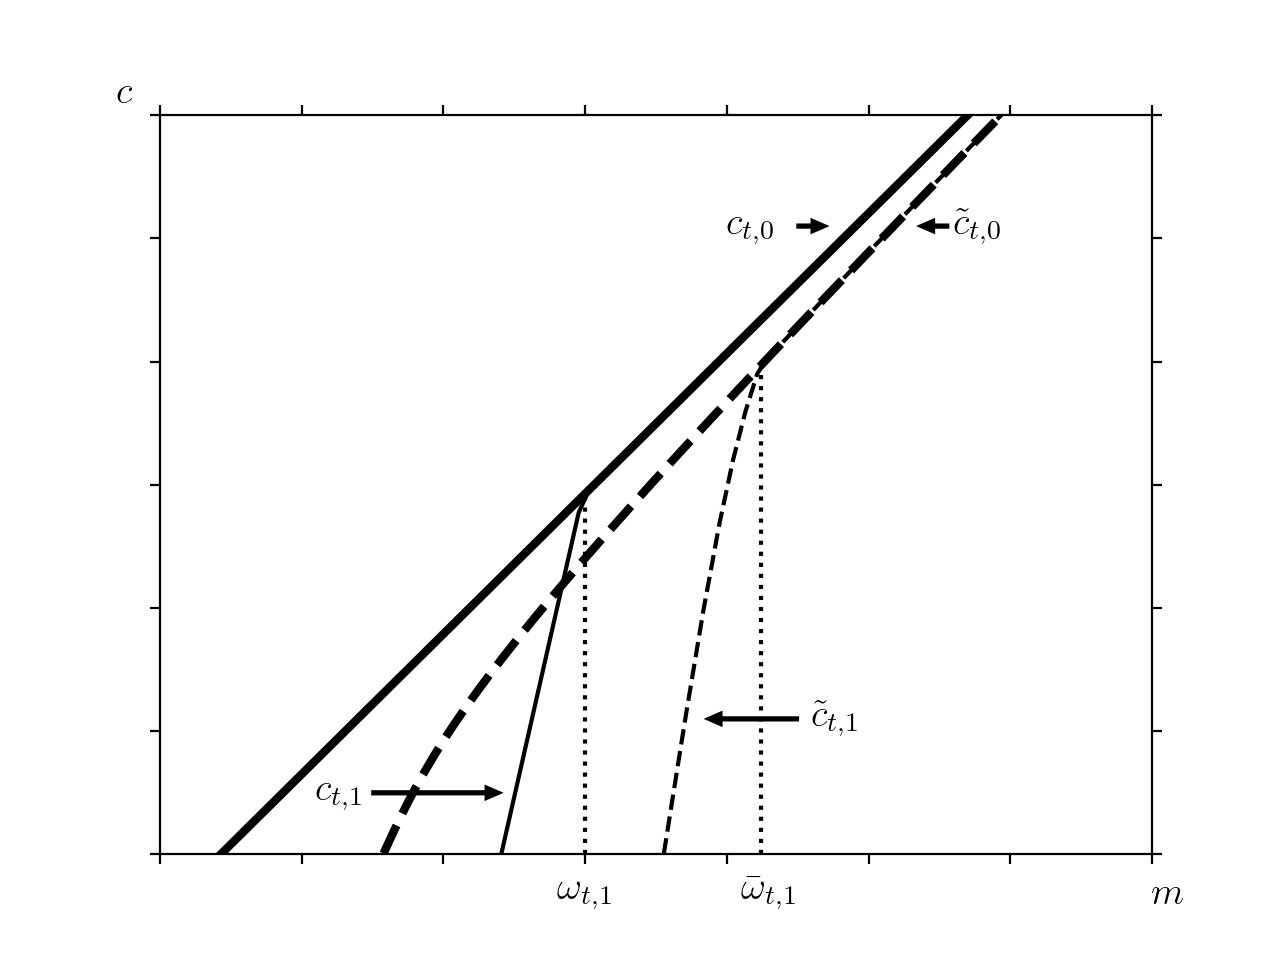
\includegraphics[width=.95\textwidth]{\FigDir/ConsWithWithoutConstrAndRisk}}

\caption{Consumption Functions with and without a Constraint and a Risk}
{\footnotesize \begin{singlespace} {\emph{Notes:} $c_{t,0}$ is the consumption function with no constraint and no risk, $\tilde{c}_{t,0}$ is the consumption function with no constraint and a risk that is realized at the beginning of period $t+1$, $c_{t,1}$ is the consumption function with one constraint in period $t+1$ and no risk, and $\tilde{c}_{t,1}$ is the consumption function with one constraint in period $t+1$ and a risk that is realized at the beginning of period $t+1$. The figure illustrates that the vertical distance between $c_{t,1}$ and $\tilde{c}_{t,1}$ is always greater than the vertical distance between $c_{t,0}$ and $\tilde{c}_{t,0}$ for $w < \bar{\omega}_{t,1}$. }  \end{singlespace}}
\label{fig:SolveConstrCompare4Cases}
\end{figure}
The thinner loci reflect behavior of consumers who face the future constraint, and the dashed loci reflect behavior of consumers who face the immediate risk. For levels of wealth above $\wAlt_{t,1}$ where the future constraint stops impinging on current behavior for perfect foresight consumers, behavior of the constrained and unconstrained perfect foresight consumers is the same. Similarly, $\tilde{c}_{t,1}(w_{t}) = \tilde{c}_{t,0}(w_{t})$ for levels of wealth above ${\bar{\wAlt}}_{t,1}$ beyond which the probability of the future constraint binding is zero. For both constrained and unconstrained consumers, the introduction of the risk reduces the level of consumption (the dashed loci are below their solid counterparts). The significance of Theorem \ref{thm:riskandconstraints} in this context is that for levels of wealth below ${\bar{\wAlt}}_{t,1}$, the vertical distance between the solid and the dashed loci is greater for the constrained (thin line) than for the unconstrained (thick line) consumers, because of the interaction between the liquidity constraint and the precautionary motive.


\subsection{A More General Result?}
The result in Theorem \ref{thm:riskandconstraints} is limited to the effects of an additional constraint when a household faces income risk that is realized at the beginning of period $t+1$. Intuition might suggest that this could be generalized to a proposition that  precautionary saving increases if we for example impose an immediate constraint or an earlier risk, or generally impose multiple constraints or risks. However, it turns out that the answer is ``not necessarily'' to all these possible scenarios. In this subsection, we explain why we cannot derive more general results.


To describe these results, we need to develop a last bit of notation.  We define, $c_{t,n}^{m}$, as the consumption function in period $t$ assuming that the first $n$ constraints and the first $m$ risks have been imposed, counting risks, like constraints, backwards from period $T$.  Thus, relating our new notation to our previous usage, $c_{t,n}^{0}=c_{t,n}$ because 0 risks have been imposed. All other functions are defined correspondingly, e.g. $\Omega_{t,n}^{m}$ is the end-of-period-$t$ value function assuming the first $n$ constraints and $m$ risks have been imposed. We will continue to use the notation $\tilde{c}_{t,n}$ to designate the effects of imposition of a single immediate risk (realized at the beginning of period $t+1$).

Suppose now there are $m$ future risks that will be realized between $t$ and $T$. One might hope to show that, at any $w$, the precautionary effect of imposing all risks in the presence of all constraints would be greater than the effect of imposing all risks in the absence of any
constraints:
\begin{equation}
  c_{t,n}^{0}(w) - c_{t,n}^{m}(w) \geq c_{t,0}^{0}(w) - c_{t,0}^{m}(w).\label{eq:nottrue}
\end{equation}
Such a hope, however, would be in vain.  In fact, we will now show that even the considerably weaker condition, involving only the single risk $\zeta_{t+1}$ and all constraints, $c_{t,n}^{0}(w) - c_{t,n}^{1}(w) \geq c_{t,0}^{0}(w) - c_{t,0}^{1}(w),$ can fail to hold for some $w$.


\subsubsection{An Immediate Constraint}\label{subsubsec:ImmediateConstr}


Consider a situation in which $n$ constraints apply in between $t$ and $T$. Since $c_{t,n-1}$ designates the consumption rule that will be optimal prior to imposing the period-$t$ constraint, the consumption rule imposing all constraints will be
\begin{eqnarray}
c_{t,n}(w) & = & \min[c_{t,n-1}(w),w].
\end{eqnarray}
Now define the level of wealth below which the period $t$ constraint binds for a consumer not facing the risk as ${\wAlt}_{t,n}.$ For values of wealth $w \geq {\wAlt}_{t,n},$ analysis of the effects of the risk is identical to analysis in the previous subsection where the first $n-1$ constraints were imposed. For levels of wealth $w < {\wAlt}_{t,n}$, we have $c^{1}_{t,n}(w) = c_{t,n}(w)=w$ (for the simple $c \leq w$
constraint; a corresponding point applies to the more sophisticated form of constraint); that is, for consumers with wealth below ${\wAlt}_{t,n}$, the introduction of the risk in period $t+1$ has no effect on consumption in $t$, because for these levels of wealth the constraint at the end of $t$ has the effect of hiding the risk from view (they were constrained before the risk was imposed and remain constrained afterwards). Thus for agents for whom inequality \eqref{eq:ineq} in Theorem \ref{thm:riskandconstraints} holds strictly in the absence of the constraint at $t$, at levels of wealth below ${\wAlt}_{t,n}$, the precautionary effect of the risk is wiped out.

\subsubsection{An Earlier Risk}\label{subsubsec:AnEarlierRisk}

Consider now the question of how the addition of a risk $\zeta_{t}$ that will be realized at the beginning of period $t$ affects the consumption function at the beginning of period $t-1$, in the absence of any constraint at the beginning of period $t$.

The question at hand is then whether we can say that
\begin{eqnarray}
  \label{eq:earlierrisk}
  c_{t-1,0}^{1}(w)-c_{t-1,0}^{2}(w) & \geq & c_{t-1,0}^0(w)-c^{1}_{t-1,0}(w);
\end{eqnarray}
that is, does the introduction of the risk $\zeta_{t}$ have a greater precautionary effect on consumption in the presence of the subsequent risk $\zeta_{t+1}$ than in its absence?

The answer again is ``not necessarily.''  To see why, we present an example in Appendix \ref{app:similar} of a CRRA utility problem in which in a certain limit the introduction of a risk produced an effect on the consumption function that is indistinguishable from the effect of a liquidity constraint.  If the risk $\zeta_{t}$ is of this liquidity-constraint-indistinguishable form, then the logic of the previous subsection applies: For some levels of wealth, the introduction of the risk at $t$ can weaken the precautionary effect of any risks at $t+1$ or later.

\subsection{What Can Be Said?}\label{subsubsec:WhatCanBeSaid}



It might seem that the previous subsection implies that little useful can be said about the precautionary effects of introducing a new risk in the presence of preexisting constraints and risks. It turns out, however, that there is at least one strong result.

\begin{theorem}\label{thm:CCandPS}
	Consider an agent who has a utility function with $u'> 0$, $u''< 0$, $u''' > 0$, and non-increasing absolute prudence ($-u'''/u''$). Then the introduction of a risk $\zeta_{t+1}$ has a greater precautionary effect on period $t$ consumption in the presence of all future risks and constraints than in the absence of any future risks and constraints, i.e.
	\begin{eqnarray}
	c_{t,n}^{m-1}(w) - c_{t,n}^{m}(w) & > & c_{t,0}^0(w)-c^{1}_{t,0}(w) \label{eq:whatcanbesaid}
	\end{eqnarray}
    at levels of period-$t$ wealth $w$ such that in the absence of the new risk the consumer is not constrained in the current period $(c_{t,n}^{m-1}(w) > w)$ and in the presence of the risk there is a positive probability that some future constraint will bind.
\end{theorem}

Appendix \ref{app:CCandPS} presents the proof. It seems to us that a fair summary of this theorem is that in most circumstances the presence of future constraints and risks does increase the amount of precautionary saving induced by the introduction of a given new risk.  The primary circumstance under which this should not be expected is for levels of wealth at which the consumer was constrained even in the absence of the new risk. There is no guarantee that the new risk will produce a sufficiently intense precautionary saving motive to move the initially-constrained consumer off his constraint.  If it does, the effect will be precautionary, but it is possible that no effect will occur.

